\item \points{15} {\bf Poisson Regression}

In this question we will construct another kind of a commonly used GLM, which is called Poisson Regression. In a GLM, the choice of the exponential family distribution is based on the kind of problem at hand. If we are solving a classification problem, then we use an exponential family distribution with support over discrete classes (such as Bernoulli, or Categorical). Similarly, if the output is real valued, we can use Gaussian or Laplace (both are in the exponential family). Sometimes the desired output is to predict counts. E.g., predicting the number of emails expected in a day, the number of customers expected to enter a store in the next hour, etc. based on input features (also called covariates). You may recall that a probability distribution with support over integers (i.e. counts) is the Poisson distribution, and it also happens to be in the exponential family.

In the following sub-problems, we will start by showing that the Poisson distribution is in the exponential family, derive the functional form of the hypothesis, derive the update rules for training models, and finally using the provided dataset to train a real model and make predictions on the test set.

\begin{enumerate}
	\item \subquestionpointswritten{2} Consider the Poisson distribution parameterized by $\lambda$:
%
\begin{equation*}
  p(y; \lambda) = \frac{e^{-\lambda}\lambda^y}{y!}.
\end{equation*}
%
(Here $y$ has positive integer values and $y!$ is the factorial of $y$. ) Show that the Poisson distribution is in the exponential family, and clearly state the values for $b(y)$, $\eta$, $T(y)$, and $a(\eta)$.\\

{\bf BEGIN PROOF HERE}\\[20pt]

\begin{flalign*}
  p(y; \lambda) \\
  &= \frac{e^{-\lambda}\lambda^y}{y!}  \\
  &= \exp \left(-\lambda + y\log(\lambda) - \log(y!) \right) \\
  &= \frac{\exp \left(y\log(\lambda) - \lambda \right)}
  	{\exp \left( \log(y!) \right)} \\
  &= \frac{1}{y!} \exp \left(\log(\lambda)y - \lambda \right)\\\\\\
  b(y) &= \frac{1}{y!} \\
  \eta &=  \log(\lambda) \\
  T(y) &= y \\
  a(\eta) &= \lambda = e^\eta
	\\[50pt]
\end{flalign*}

{\bf END PROOF}\\

\ifnum\solutions=1{
  \input{poisson/01-exponential-sol}
}\fi

	\item \subquestionpointswritten{1} Consider performing regression using a GLM model with a Poisson response variable.  What is the canonical response function for the family?  (You may use the fact that a Poisson random variable with parameter $\lambda$ has mean $\lambda$.)\\[20pt]


\begin{flalign*}
  \mathbb{E}[T(y); \eta] &= \mathbb{E}[y; \eta]  \\
  \mathbb{E}[y; \eta] &= \lambda \\
  &= e^\eta
	\\[50pt]
\end{flalign*}



\ifnum\solutions=1{
	\input{poisson/02-response-fn-sol}
}\fi

	\item \subquestionpointswritten{7} For a training set $\{(x^{(i)}, y^{(i)});\, i=1,\ldots,\nexp\}$, let the log-likelihood of an example be $\log p(y^{(i)} | x^{(i)}; \theta)$. By taking the derivative of the log-likelihood with respect to $\theta_j$, derive the stochastic gradient ascent update rule for learning using a GLM model with Poisson responses $y$ and the canonical response function.\\

{\bf BEGIN PROOF HERE}\\

The log-likelihood of an example $(x^{(i)}, y^{(i)})$ is defined as $\ell(\theta) = \log p(y^{(i)} | x^{(i)}; \theta)$. To derive the stochastic gradient ascent rule, use the results in part (a) and the standard GLM assumption that $\eta = \theta^Tx$.
\begin{flalign*}
	\frac{\partial \ell(\theta)}{\partial \theta_j}
	&= \frac{\partial \log p(y^{(i)} | x^{(i)}; \theta)}{\partial \theta_j}\\
	&= \frac {\partial \log \left({\frac{1}{y^{(i)}!} \exp(\eta^T y^{(i)} -
	e^\eta)}\right)} {\partial \theta_j}\\\\
    &= \frac {\partial}{\partial \theta_j} \left(
    	\log(\frac{1}{y!}) +\eta^T y^{(i)} -e^\eta
    	\right) \\
    &= \frac {\partial}{\partial \theta_j} \left(
    	\log(\frac{1}{y!}) +\theta^Tx^{(i)} y^{(i)} -e^{\theta^Tx^{(i)}}
    	\right) \\
    &= y^{(i)}x^{(i)} - e^{\theta^Tx^{(i)}}x^{(i)} \\
    &= \left(y^{(i)} - e^{\theta^Tx^{(i)}} \right)x^{(i)}
    & & & & &\\[50pt]
\end{flalign*}

The stochastic gradient ascent update rule is
%
\begin{equation*}
\theta_j := \theta_j + \alpha \frac{\partial \ell(\theta)}{\partial \theta_j},
\end{equation*}
%
which reduces here to:\\[50pt]
$ \theta_j := \theta_j + \alpha\left(y^{(i)} - e^{\theta^Tx^{(i)}} \right)x^{(i)} $ \\[20pt]
{\bf END PROOF}\\


\ifnum\solutions=1{
  \input{poisson/03-gd-update-sol}
}\fi

	\item \subquestionpointscoding{5}

Consider a website that wants to predict its daily traffic. The website owners have collected a dataset of past traffic to their website, along with some features which they think are useful in
predicting the number of visitors per day. The dataset is split into train/valid sets and the starter code is provided in the following files:
\begin{center}
    \begin{itemize}
        \item 	\texttt{poisson/src/{train,valid}.csv}
        \item   \texttt{poisson/src/poisson.py}
    \end{itemize}
\end{center}
We will apply Poisson regression to model the number of visitors per day. Note that applying Poisson regression in particular assumes that the data follows a Poisson distribution whose natural parameter is a linear combination of the input features (\emph{i.e.,} $\eta = \theta^T x$). In \texttt{poisson/src/poisson.py}, implement Poisson regression for this dataset and use \emph{full batch gradient ascent} to maximize the log-likelihood of $\theta$. For the stopping criterion, check if the change in parameters has a norm smaller than a small value such as $10^{-5}$.

Using the trained model, predict the expected counts for the \textbf{validation set}.  To verify a correct implementation, consider creating a scatter plot between the true counts vs predicted counts (on the validation set). In the scatter plot, let x-axis be the true count and y-axis be the corresponding predicted expected count. Note that the true counts are integers while the expected counts are generally real values.\\

Your plot should look similar to the following:

\begin{figure}[H]
	\centering
	\vspace{-2mm}
	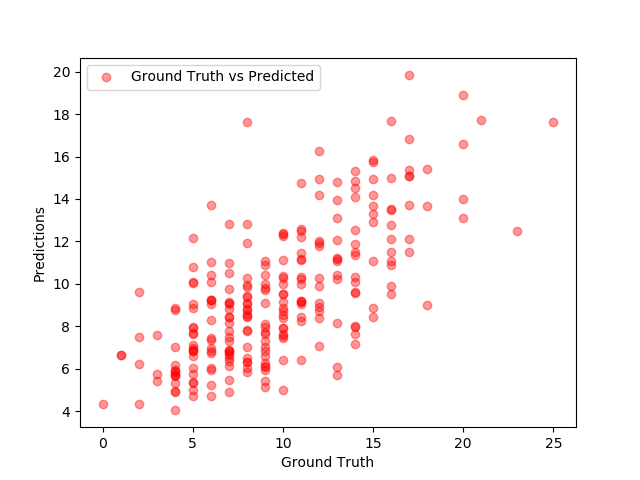
\includegraphics[width=0.65\linewidth]{poisson/src/poisson_val.png}
	\caption{Ground Truth vs Prediction plot on the validation set (Note: This is for reference only.  You are not required to submit a plot.)}
\end{figure}


\ifnum\solutions=1 {
  \input{poisson/04-regression-sol}
} \fi

\end{enumerate}
